%%%%%%%%%%%%%%%%%%%%%%%%%%%%%%%%%%%%%%%%%%%%%%%%%%%%%%%%%%%%%%%%%%%%%%%%%%%%%
%  enslyonstage.tex — Guide d'utilisation du template ENSLyonStage v2.2
%
%  Compilez avec : pdflatex enslyonstage → biber enslyonstage → pdflatex enslyonstage  (×2 pour ToC et \autoref{})
%%%%%%%%%%%%%%%%%%%%%%%%%%%%%%%%%%%%%%%%%%%%%%%%%%%%%%%%%%%%%%%%%%%%%%%%%%%%%

\documentclass[12pt, a4paper]{article}

% ── Encodage et langue ─────────────────────────────────────────────────────
\usepackage[utf8]{inputenc}
\usepackage[T1]{fontenc}
\usepackage[french]{babel}
\usepackage{csquotes}

% ── Bibliographie (même style que enslyonstage.cls) ───────────────────────
\usepackage[style=numeric-comp,
            sorting=none,
            backend=biber,
            maxbibnames=99,
            doi=false,
            isbn=false,
            url=false,
            eprint=false]{biblatex}
\addbibresource{references.bib}
\AtBeginDocument{%
  \renewcommand{\bibfont}{\small}%
  \setlength{\bibitemsep}{0pt}%
  \setlength{\bibhang}{0pt}%
}

% ── Géométrie ──────────────────────────────────────────────────────────────
\usepackage[margin=25mm,
            headheight=15pt]{geometry}

% ── Polices ────────────────────────────────────────────────────────────────
\usepackage{palatino}
\usepackage{mathpazo}
\usepackage{amssymb}

% ── Couleurs ───────────────────────────────────────────────────────────────
\usepackage{xcolor}
% Thème clair pour les boîtes de code (style guide-latex-fr)
\definecolor{darkbg}     {HTML}{F5EFE7}  % fond code — crème chaude
\definecolor{codegray}   {HTML}{2C1E14}  % texte de base — brun très foncé
\definecolor{codepurple} {HTML}{7B2F8B}  % \begin \end \newcommand — violet foncé
\definecolor{codeblue}   {HTML}{1A5C9E}  % commandes ENS — bleu (= tipsblue)
\definecolor{codegreen}  {HTML}{2E7D32}  % strings — vert foncé
\definecolor{codeyellow} {HTML}{9A6400}  % (réservé) — ambre foncé
\definecolor{codecomment}{HTML}{8B7355}  % commentaires — gris brun chaud
\definecolor{ENSorange}  {HTML}{E14D17}
\definecolor{ENSaccent}  {HTML}{E07820}
\definecolor{ENSbg}      {HTML}{FDF5EC}
\definecolor{tipsblue}   {HTML}{1A5C9E}
\definecolor{tipsbg}     {HTML}{EDF4FB}
\definecolor{warnred}    {HTML}{A62020}
\definecolor{warnbg}     {HTML}{FBF0F0}
\definecolor{resultbg}   {HTML}{FFFFFF}  % résultat — blanc pur

% ── Coloration syntaxique ──────────────────────────────────────────────────
\usepackage{listings}
\lstdefinestyle{latexcode}{
  language=[LaTeX]TeX,
  backgroundcolor=\color{darkbg},
  basicstyle=\ttfamily\small\color{codegray},
  keywordstyle=\color{codepurple}\bfseries,
  commentstyle=\color{codecomment}\itshape,
  stringstyle=\color{codegreen},
  breaklines=true,
  breakatwhitespace=false,
  tabsize=2,
  showstringspaces=false,
  columns=flexible,
  keepspaces=true,
  frame=none,
  numbers=left,
  numberstyle=\tiny\ttfamily\color{codecomment},
  numbersep=8pt,
  xleftmargin=22pt,
  xrightmargin=6pt,
  aboveskip=0pt,
  belowskip=0pt,
  % Caractères français — literate remplace les séquences UTF-8 AVANT le
  % traitement verbatim (contournement de la limitation de listings)
  literate=
    {à}{{\`a}}1 {â}{{\^a}}1 {ä}{{\"a}}1
    {é}{{\'e}}1 {è}{{\`e}}1 {ê}{{\^e}}1 {ë}{{\"e}}1
    {î}{{\^i}}1 {ï}{{\"i}}1
    {ô}{{\^o}}1 {ö}{{\"o}}1
    {ù}{{\`u}}1 {û}{{\^u}}1 {ü}{{\"u}}1
    {ç}{{\c c}}1 {œ}{{\oe{}}}1 {æ}{{\ae}}1
    {É}{{\'E}}1 {È}{{\`E}}1 {Ê}{{\^E}}1 {Ë}{{\"E}}1
    {À}{{\`A}}1 {Â}{{\^A}}1 {Ä}{{\"A}}1
    {Î}{{\^I}}1 {Ï}{{\"I}}1
    {Ô}{{\^O}}1 {Ö}{{\"O}}1
    {Ù}{{\`U}}1 {Û}{{\^U}}1 {Ü}{{\"U}}1
    {Ç}{{\c C}}1 {Œ}{{\OE{}}}1 {Æ}{{\AE}}1
    {→}{{$\rightarrow$}}1 {←}{{$\leftarrow$}}1
    {—}{{---}}1 {–}{{--}}1
    {°}{{$^\circ$}}1
    {≤}{{$\leq$}}1 {≥}{{$\geq$}}1
    {×}{{$\times$}}1 {±}{{$\pm$}}1
    {µ}{{$\mu$}}1 {μ}{{$\mu$}}1,
  % Commandes spécifiques au template en surbrillance bleue
  morekeywords={[2]titre,auteur,master,domaine,datedebut,datefin,
    laboratoire,tuteurstage,tuteurENS,abstracts,abstractimage,keywords,
    nombredemots,stagesanterieurs,stagerow,logoENS,logoformation,logoLabo,
    fairepagedegarde,faireabstract,insererfigure,inserersuppfig,biblio,
    FloatBarrier,balance,TODO,NOTE,crefcolor,
    coinhautgauche,coinhautdroit,coinbasgauche,coinbascentre,coinbasdroit,
    lettrine,SI,si,SIrange,num,ce,cite,citeauthor,citeyear,
    autoref,cref,addbibresource,hyphenation},
  keywordstyle={[2]\color{codeblue}\bfseries},
}

% ── tcolorbox ──────────────────────────────────────────────────────────────
\usepackage{tcolorbox}
\tcbuselibrary{listings, skins, breakable, most}
% Débordement sur les marges : changepage fournit adjustwidth qui redéfinit
% \linewidth à l'intérieur — bien plus fiable que enlarge left/right by
\usepackage{changepage}

% Boîte principale : code à gauche | résultat à droite
%
% Architecture : newtcolorbox (PAS newtcblisting) + lstlisting explicite.
% Voir commentaire de session pour les raisons techniques.
%
% Structure d'un bloc demo :
%   \begin{demo}
%   \begin{lstlisting}[style=latexcode]
%   ...code...
%   \end{lstlisting}
%   \tcblower
%   ...résultat compilé...
%   \end{demo}
%
% Débordement sur les marges — architecture en deux couches :
%
%   demo       = NewDocumentEnvironment qui enveloppe adjustwidth + demoinner
%   demoinner  = vrai tcolorbox (sidebyside, \tcblower, etc.)
%
%   On NE PEUT PAS mettre adjustwidth dans before={}/after={} de tcolorbox :
%   adjustwidth est un environnement list en interne ; ses groupes entrent en
%   collision avec les groupes internes de tcolorbox (tcb@drawing) et causent
%   des erreurs "ended by \end{list} / \end{adjustwidth}".
%
%   Solution : adjustwidth enveloppe demoinner de l'extérieur, comme un vrai
%   environnement LaTeX imbriqué. À l'intérieur, \linewidth = 200mm, donc
%   lefthand width = 3\linewidth/5 - 3mm ≈ 117mm → split 60/40 exact.

\newtcolorbox{demoinner}[1][]{
  enhanced,
  sidebyside,
  sidebyside align=top seam,
  lefthand width=\dimexpr3\linewidth/5-3mm\relax,
  sidebyside gap=3mm,
  colback=darkbg,
  colbacklower=resultbg,
  colframe=ENSorange!80,
  left=2pt, right=2pt, top=4pt, bottom=4pt,
  fonttitle=\sffamily\bfseries\small,
  #1
}

\NewDocumentEnvironment{demo}{O{}}{%
  \begin{adjustwidth}{-20mm}{-20mm}%
  \noindent%
  \begin{demoinner}[#1]%
}{%
  \end{demoinner}%
  \end{adjustwidth}%
}

% Astuce (fond bleu clair)
\newtcolorbox{astuce}{
  enhanced,
  colback=tipsbg,
  colframe=tipsblue,
  leftrule=4pt, rightrule=0.4pt, toprule=0.4pt, bottomrule=0.4pt,
  arc=2pt, left=8pt,
  fonttitle=\sffamily\bfseries\color{tipsblue},
  title={Astuce},
  attach title to upper={\ —\ },
}

% Attention (fond rouge clair)
\newtcolorbox{attention}{
  enhanced,
  colback=warnbg,
  colframe=warnred,
  leftrule=4pt, rightrule=0.4pt, toprule=0.4pt, bottomrule=0.4pt,
  arc=2pt, left=8pt,
  fonttitle=\sffamily\bfseries\color{warnred},
  title={Attention},
  attach title to upper={\ —\ },
}

% ── Simulation de l'apparence ENSLyonStage ────────────────────────────────
% Commandes utilisées dans la colonne "résultat" des boîtes demo

% Citation en exposant coloré
\newcommand{\simcite}[1]{%
  \textsuperscript{\textcolor{ENSorange}{\bfseries[#1]}}}

% Lien coloré (autoref, crefcolor)
\newcommand{\simlink}[1]{\textcolor{ENSorange}{#1}}

% En-tête de section (fond coloré)
\newcommand{\simsection}[2][1]{%
  \colorbox{ENSbg}{\parbox{\dimexpr\linewidth-2\fboxsep\relax}{%
    \centering\color{ENSorange}\sffamily\bfseries\normalsize
    #1.\enspace #2}}\par}

% En-tête de section non numérotée (sans numéro ni point)
\newcommand{\simsectionstar}[1]{%
  \colorbox{ENSbg}{\parbox{\dimexpr\linewidth-2\fboxsep\relax}{%
    \centering\color{ENSorange}\sffamily\bfseries\normalsize
    #1}}\par}

% Commande \BibTeX stylisée
\newcommand{\BibTeX}{\textsc{Bib}\TeX}

% En-tête de subsection
\newcommand{\simsubsection}[2][1.1]{%
  {\color{ENSorange}\sffamily\bfseries #1\enspace #2}\par}

% Titre de paragraph (run-in)
\newcommand{\simparagraph}[1]{%
  {\color{ENSorange}\sffamily\bfseries\small #1}\ }

% Swatch de couleur pour le tableau des thèmes : \sw{RRGGBB}{nom}
\newcommand{\sw}[2]{%
  \colorbox[HTML]{#1}{\rule{0pt}{5.5pt}\hspace{9pt}}~\textbf{\small #2}}

% Placeholder de figure avec légende
\newcommand{\simfigbox}[2][fig.pdf]{%
  \begin{center}
    \fbox{\parbox{0.78\linewidth}{\centering\vspace{8pt}%
      \textcolor{gray!60}{\rule{2.2cm}{1.4cm}}\\[4pt]
      {\tiny\ttfamily\color{gray} #1}\vspace{8pt}}}\\[4pt]
    {\small\textcolor{ENSorange}{\textbf{Figure~1.}}\ #2}%
  \end{center}}

% ── Hyperliens ─────────────────────────────────────────────────────────────
\usepackage[colorlinks, linkcolor=ENSorange, urlcolor=ENSaccent,
            citecolor=ENSorange, pdftitle={Guide ENSLyonStage v2.2},
            pdfauthor={ENS de Lyon}]{hyperref}

% ── En-têtes et pieds de page ─────────────────────────────────────────────
\usepackage{fancyhdr}
\pagestyle{fancy}
\fancyhf{}
\fancyhead[L]{\small\sffamily\color{ENSorange} Guide \texttt{ENSLyonStage} v2.2}
\fancyhead[R]{\small\sffamily\leftmark}
\fancyfoot[C]{\small\sffamily\thepage}
\renewcommand{\headrulewidth}{0.4pt}
\renewcommand{\headrule}{{\color{ENSorange}\hrule width\headwidth height 0.4pt}}

% ── Divers ─────────────────────────────────────────────────────────────────
\usepackage{lettrine}
\renewcommand{\LettrineFontHook}{\color{ENSorange}}
\usepackage{tikz}
\usepackage{graphicx}
\graphicspath{{figures/}{logos/}}
\usepackage{booktabs}
\usepackage{array}
% ── siunitx + mhchem (pour les demos droite) ──────────────────────────────
\usepackage{siunitx}
\sisetup{inter-unit-product=\cdot}
\DeclareSIUnit{\Molar}{M}
\DeclareSIUnit{\rpm}{rpm}
\usepackage[version=4]{mhchem}
% Colonne centrée avec retour à la ligne automatique
\newcolumntype{C}[1]{>{\centering\arraybackslash}p{#1}}
\usepackage{enumitem}
\usepackage{microtype}
\usepackage{lastpage}
\setcounter{tocdepth}{2}

% Espacement des sections
\usepackage{titlesec}
\titleformat{\section}{\color{ENSorange}\Large\bfseries\sffamily}{\thesection.}{0.5em}{}
  [\color{ENSorange}\rule{\linewidth}{0.6pt}]
\titleformat{\subsection}{\color{ENSorange}\large\bfseries\sffamily}{\thesubsection}{0.5em}{}
\titleformat{\subsubsection}{\bfseries\sffamily}{\thesubsubsection}{0.5em}{}

% Espacement TOC
\usepackage{titletoc}
% \contentsmargin{right} réserve de l'espace pour les numéros de page à droite.
% Pour les sections : label "14" ≈ 1.5pc → OK.
% Pour les subsections : label "14.3" ≈ 2pc → augmenté de 1.5pc à 2pc,
%   indent total 3pc → 3.5pc pour conserver l'alignement du texte.
\contentsmargin{2em}
\titlecontents{section}[1.5pc]{\addvspace{4pt}\bfseries\sffamily}
  {\contentslabel{1.5pc}}{}{\hfill\thecontentspage}
\titlecontents{subsection}[3.5pc]{\small\sffamily}
  {\contentslabel{2pc}}{}{\titlerule*[.5pc]{.}\thecontentspage}

%%%%%%%%%%%%%%%%%%%%%%%%%%%%%%%%%%%%%%%%%%%%%%%%%%%%%%%%%%%%%%%%%%%%%%%%%%%%%
\begin{document}
%%%%%%%%%%%%%%%%%%%%%%%%%%%%%%%%%%%%%%%%%%%%%%%%%%%%%%%%%%%%%%%%%%%%%%%%%%%%%

% ── Page de titre ──────────────────────────────────────────────────────────
\begin{titlepage}
  \thispagestyle{empty}
  \centering
  \vspace*{1.8cm}
  {\color{ENSorange}\rule{0.85\linewidth}{1.2pt}}\par\vspace{0.5cm}
  {\Huge\bfseries\sffamily Guide d'utilisation\par}
  \vspace{0.35cm}
  {\LARGE\sffamily du template \texttt{ENSLyonStage}\par}
  \vspace{0.5cm}
  {\color{ENSorange}\rule{0.85\linewidth}{1.2pt}}\par\vspace{0.5cm}
  {\large\itshape Rapports de stage M1/M2 Biosciences — ENS de Lyon\par}
  \vspace{0.25cm}
  {\large Version 2.2 — Septembre 2026\par}
  \vspace{0.25cm}
  {Adama \textsc{Mbaye}\par}
  \vspace{0.9cm}
  %
  % ── Plot « Effort vs complexité » ─────────────────────────────────────────
  \begin{tikzpicture}[>=stealth, line width=1.4pt, font=\small\sffamily]
    % ── Axes ────────────────────────────────────────────────────────────────
    \draw[->] (0,0) -- (7.5,0)
      node[right, font=\footnotesize\sffamily, align=left]
      {Complexité et\\ taille du rapport};
    \draw[->] (0,0) -- (0,5.6);
    % Label Y rotaté 90° sur le côté gauche
    \node[rotate=90, anchor=center, font=\footnotesize\sffamily]
      at (-0.55, 2.8) {Effort et temps requis};
    % ── Ligne "Impossible à faire" (rouge) ──────────────────────────────────
    % Position y=4.8, texte centré au-dessus
    \draw[red!80!black, line width=1.6pt] (0.15,4.8) -- (7.3,4.8);
    \node[red!80!black, font=\small\bfseries\sffamily, anchor=center]
      at (3.6, 5.12) {Impossible à faire};
    % ── Courbe Word (orange pointillée, exponentielle) ───────────────────────
    % f(x) = 0.2·exp(0.65·x)
    % f(0)=0.20 (part bas) ; f(3.5)≈1.95 (croise LaTeX) ; f(4.89)≈4.80 (limite)
    \draw[orange!90!black, dashed, smooth]
      plot[domain=0:4.89, samples=60] (\x, {0.2*exp(0.65*\x)});
    \node[orange!90!black, font=\small\bfseries\sffamily] at (3.2, 0.78) {Word};
    % ── Courbe LaTeX (vert, croissance lente) ────────────────────────────────
    % g(x) = 1.2 + 0.12·x^1.5  (écrit x·√x pour compatibilité PGF)
    % g(0)=1.20 (part haut) ; g(3.5)≈1.99 (croise Word) ; g(7)≈3.42 (sous limite)
    \draw[green!55!black, smooth]
      plot[domain=0:7.2, samples=80] (\x, {1.2 + 0.12*\x*sqrt(\x)});
    \node[green!55!black, font=\small\bfseries\sffamily] at (6.3, 3.7) {\LaTeX};
  \end{tikzpicture}
  %
  \vfill
  \begin{tcolorbox}[colback=ENSbg, colframe=ENSorange!40, width=0.85\linewidth,
                    left=8pt, right=8pt]
    \small\sffamily
    Ce document explique comment utiliser toutes les commandes du template.
    Chaque boîte présente le \textbf{code} à gauche et le \textbf{rendu visuel}
    à droite. Pour voir le rendu visuel d'un rapport complet, consulter
    \texttt{enslyonstage-exemple.tex} (démonstration visuelle uniquement,
    pas un modèle de fond scientifique).\\[4pt]
    \textcolor{ENSaccent}{\url{https://github.com/adammbaye/enslyonstage}}
  \end{tcolorbox}
\end{titlepage}

% ── Table des matières ─────────────────────────────────────────────────────
\tableofcontents
\clearpage

% ═══════════════════════════════════════════════════════════════════════════
\section{Introduction}
% ═══════════════════════════════════════════════════════════════════════════

Le template \textbf{ENSLyonStage} est une classe \LaTeX{} sur-mesure pour
les rapports de stage M1 et M2 Biosciences de l'ENS de Lyon. Il génère
automatiquement la page de garde officielle, les en-têtes et pieds de page,
et formate le texte conformément aux exigences de l'école.

\subsection{Fichiers du template}

\begin{center}
\begin{tabular}{lp{8.5cm}}
  \toprule
  \textbf{Fichier} & \textbf{Rôle} \\
  \midrule
  \texttt{enslyonstage-gabarit.tex}  & \textbf{Votre rapport} — à compléter et compiler \\
  \texttt{enslyonstage-exemple.tex}  & Démonstration visuelle du rendu — basée sur un vrai rapport M1 publié sur Zenodo (\url{https://doi.org/10.5281/zenodo.21631816}) ; ne pas prendre comme modèle de fond scientifique \\
  \texttt{enslyonstage.cls}    & Classe \LaTeX{} du template (ne pas modifier) \\
  \texttt{references.bib}      & Exemple de base de données bibliographique \\
  \texttt{figures/}            & Vos figures (PDF, PNG, JPG\ldots) \\
  \texttt{logos/}              & Logos du labo et Bandeaux ENS (\texttt{hautdepage.pdf},
                                 \texttt{basdepage.pdf}, \texttt{logo\_ens.pdf}\ldots) \\
  \bottomrule
\end{tabular}
\end{center}

\subsection{Exigences ENS de Lyon}

\begin{center}
\begin{tabular}{lC{3.8cm}C{3.8cm}}
  \toprule
  & \textbf{M1} & \textbf{M2} \\
  \midrule
  Mots (hors légendes et références) & $\leqslant$ 5\,000 ($\pm$\,10\,\%) & $\leqslant$ 4\,000 ($\pm$\,10\,\%) \\
  Figures + tableaux                 & $\leqslant$ 6 & $\leqslant$ 5 \\
  Références                         & \multicolumn{2}{C{7.6cm}}{$\leqslant$ 35} \\
  Titre                              & \multicolumn{2}{C{7.6cm}}{$\leqslant$ 125 caractères} \\
  Abstract                           & \multicolumn{2}{C{7.6cm}}{150–200 mots, en anglais, sans référence} \\
  \bottomrule
\end{tabular}
\end{center}

% ═══════════════════════════════════════════════════════════════════════════
\section{Démarrage rapide}
% ═══════════════════════════════════════════════════════════════════════════

\begin{enumerate}
  \item \textbf{Overleaf :} téléversez tous les fichiers du template
    (y compris \texttt{.cls}, \texttt{.bib}, les dossiers \texttt{logos/}
    et \texttt{figures/}). Overleaf détecte \texttt{enslyonstage-gabarit.tex} comme fichier
    racine et utilise \texttt{biber} automatiquement.
  \item \textbf{Métadonnées :} remplissez le préambule de
    \texttt{enslyonstage-gabarit.tex} (voir \autoref{sec:metadata}).
  \item \textbf{Figures :} ajoutez vos images dans \texttt{figures/}.
  \item \textbf{Sections :} rédigez en vous aidant de ce guide
    et de \texttt{enslyonstage-exemple.tex}.
  \item \textbf{Comptage de mots} : sur Overleaf, \texttt{Menu → Word Count}.
    Les légendes, tableaux et abstract sont exclus automatiquement.
\end{enumerate}

\begin{astuce}
  \textbf{Compilation locale :}
  \texttt{pdflatex enslyonstage-gabarit} \textrightarrow{}
  \texttt{biber enslyonstage-gabarit} \textrightarrow{}
  \texttt{pdflatex enslyonstage-gabarit}.
  Sur Overleaf, tout est géré automatiquement à chaque sauvegarde.
\end{astuce}

% ═══════════════════════════════════════════════════════════════════════════
\section{Métadonnées — page de garde}
\label{sec:metadata}
% ═══════════════════════════════════════════════════════════════════════════

Toutes les métadonnées se déclarent dans le \emph{préambule}, avant
\verb|\begin{document}|. Elles alimentent la page de garde, les en-têtes,
les pieds de page et les propriétés PDF.

\subsection{\texttt{\textbackslash titre\{\}}}

\begin{demo}
\begin{lstlisting}[style=latexcode]
\titre{Characterisation of a Novel Protein Complex Involved in Post-Transcriptional Regulation During Cellular Stress Response}
\end{lstlisting}
\tcblower
\begin{center}
  \large\bfseries
  Characterisation of a Novel Protein Complex
  Involved in Post-Transcriptional Regulation
  During Cellular Stress Response
\end{center}
\vspace{4pt}
{\footnotesize\itshape Affiché en grand sur la page de garde, dans l'en-tête droit, et dans les métadonnées PDF.}
\end{demo}

\begin{astuce}
  Pour forcer un saut de ligne dans le titre sans casser les métadonnées PDF,
  utiliser \verb|\texorpdfstring{\\}{ }| :
  \begin{lstlisting}[style=latexcode]
\titre{Première partie :\texorpdfstring{\\}{ }Deuxième partie}
  \end{lstlisting}
\end{astuce}

\begin{attention}
  Maximum \textbf{125 caractères} espaces compris (exigence ENS).
\end{attention}

\subsection{\texttt{\textbackslash auteur\{\}}}

\begin{demo}
\begin{lstlisting}[style=latexcode]
\auteur{Prénom \textsc{Nom}}
\end{lstlisting}
\tcblower
{\Large Prénom \textsc{Nom}}\\[6pt]
{\footnotesize\itshape Utiliser \texttt{\textbackslash textsc\{\}} pour les petites capitales sur le nom de famille.}
\end{demo}

\newpage

\subsection[\texttt{\textbackslash master} et \texttt{\textbackslash domaine}]{\texttt{\textbackslash master\{\}} et \texttt{\textbackslash domaine\{\}}}

\begin{demo}
\begin{lstlisting}[style=latexcode]
\master{M1}
\domaine{Molecular and Cellular Biology}
\end{lstlisting}
\tcblower
\textbf{master\{\}} : affiché sur la page de garde (``M1 Internship report'').\\[6pt]
\textbf{domaine\{\}} : affiché en pied de page gauche en petites capitales — \textsc{Molecular and Cellular Biology} — et sur la page de garde.\\[6pt]
{\footnotesize\itshape Valeurs possibles : \texttt{M1} ou \texttt{M2}.}
\end{demo}

\subsection[\texttt{\textbackslash datedebut} et \texttt{\textbackslash datefin}]{\texttt{\textbackslash datedebut\{\}} et \texttt{\textbackslash datefin\{\}}}

\begin{demo}
\begin{lstlisting}[style=latexcode]
\datedebut{02 February 2025}
\datefin{30 June 2025}
\end{lstlisting}
\tcblower
\begin{center}
\small\textbf{Internship dates:}\\
02 February 2025 -- 30 June 2025
\end{center}
{\footnotesize\itshape Format recommandé : \texttt{DD~Month~YYYY}.}
\end{demo}

\subsection{\texttt{\textbackslash laboratoire\{\}}}

\begin{demo}
\begin{lstlisting}[style=latexcode]
\laboratoire{%
  Laboratory of RNA Biology,
  Montpellier, France}
\end{lstlisting}
\tcblower
\begin{center}
\small\textbf{Laboratory:}\\
Laboratory of RNA Biology, Montpellier, France
\end{center}
{\footnotesize\itshape Le \texttt{\%} en fin de première ligne évite un espace indésirable avant la virgule.}
\end{demo}

\subsection[\texttt{\textbackslash tuteurstage} et \texttt{\textbackslash tuteurENS}]{\texttt{\textbackslash tuteurstage\{\}\{\}} et \texttt{\textbackslash tuteurENS\{\}\{\}}}

\begin{demo}
\begin{lstlisting}[style=latexcode]
% Encadrant de stage : nom, email
\tuteurstage{Dr. Jane \textsc{Smith}}
            {jane.smith@lab.fr}

% Tuteur ENS : nom, email (non affiché)
\tuteurENS{Prof. Jean \textsc{Dupont}}
          {jean.dupont@ens-lyon.fr}
\end{lstlisting}
\tcblower
\small\textbf{Supervisor:} Dr. Jane \textsc{Smith}\\
\hspace*{1.5em}{\ttfamily jane.smith@lab.fr}\\[6pt]
{\footnotesize\itshape L'email du tuteur ENS n'apparaît pas sur la page de garde mais est intégré dans les métadonnées PDF.\\ 
Pour ne pas afficher d'email, laisser le 2\textsuperscript{e} argument vide : \texttt{\{\}}.}
\end{demo}

\newpage

\subsection{\texttt{\textbackslash abstracts\{\}}}

\begin{demo}
\begin{lstlisting}[style=latexcode]
\abstracts{%
  Write your abstract here. Single
  paragraph, 150-200 words, English.
  No literature references permitted.
  Include: (1) brief background and
  question, (2) main results, (3)
  significance. [...]
}
\end{lstlisting}
\tcblower
{\footnotesize\textbf{Exigences ENS :}
\begin{itemize}[noitemsep, topsep=2pt]
  \item 150–200 mots, un seul paragraphe
  \item En anglais
  \item \textbf{Aucune} référence bibliographique
  \item Inclure : contexte, résultats principaux, signification
\end{itemize}
\medskip
\textit{L'abstract n'est \textbf{pas} compté dans les mots (exclusion automatique via directive \texttt{\%TC:} dans la classe).}}
\end{demo}

\subsection[\texttt{\textbackslash abstractimage} — optionnel]{\texttt{\textbackslash abstractimage\{\}} — abstract visuel (optionnel)}

Complète \verb|\abstracts{}| avec une image placée \emph{sous} le texte de l'abstract (schéma de principe, diagramme de workflow, résumé graphique\ldots). L'argument facultatif règle la largeur (défaut : \texttt{0.9\textbackslash textwidth}).

\begin{demo}
\begin{lstlisting}[style=latexcode]
\abstracts{%
  Non-coding RNAs (ncRNAs) are involved in an increasingly recognized number of cellular events [...]
  % --- abstract visuel ---
  \abstractimage[0.85\textwidth]{figures/visual_abstract.pdf}
}
\end{lstlisting}
\tcblower
{\footnotesize\textbf{Syntaxe :}
\begin{itemize}[noitemsep, topsep=2pt]
  \item Appel \emph{à l'intérieur} de \verb|\abstracts{}|, après le texte
  \item \texttt{[largeur]} facultatif (défaut \texttt{0.9\textbackslash textwidth})
  \item Accepte tout format reconnu par \verb|\includegraphics| (PDF, PNG, JPG\ldots)
\end{itemize}
\medskip
\textit{L'image n'est \textbf{pas} comptée dans les mots (exclusion automatique).}}
\end{demo}

\subsection{\texttt{\textbackslash keywords\{\}}}

\begin{demo}
\begin{lstlisting}[style=latexcode]
\keywords{RNA-binding proteins,
  stress granules,
  post-transcriptional regulation,
  proteomics, yeast two-hybrid}
\end{lstlisting}
\tcblower
\small\textbf{Keywords:}
\textit{RNA-binding proteins, stress granules, post-transcriptional regulation, proteomics, yeast two-hybrid}\\[6pt]
{\footnotesize\itshape 5 à 8 mots-clés, séparés par des virgules.}
\end{demo}

\newpage

\subsection{\texttt{\textbackslash nombredemots\{\}}}

\begin{demo}
\begin{lstlisting}[style=latexcode]
\nombredemots{6767}
\end{lstlisting}
\tcblower
\small\textit{Number of words:} 6\,767\\[6pt]
{\footnotesize Affiché sur la page de garde. À mettre à jour avant chaque soumission.\\
\textbf{Overleaf} : Menu → Word Count\\
\textbf{Local} : \texttt{texcount -sum -1 enslyonstage-gabarit.tex}}
\end{demo}

\subsection[\texttt{\textbackslash stagesanterieurs} et \texttt{\textbackslash stagerow}]{\texttt{\textbackslash stagesanterieurs\{\}} et \texttt{\textbackslash stagerow\{\}}}

\begin{demo}[sidebyside=false]
\begin{lstlisting}[style=latexcode]
\stagesanterieurs{
  \stagerow{L3}{Institut Pasteur, Paris}
    {Dr.~Dupont}{Virologie moléculaire}
  \stagerow{M1}{MPI Neurobiology, Munich}
    {Pr.~Schmidt}{Plasticité synaptique}
  \stagerow{M2}{}{}{}
}
\end{lstlisting}
\tcblower
\footnotesize\centering
\begin{tabular}{@{}llll@{}}
  \toprule
  \textbf{Année} & \textbf{Laboratoire} & \textbf{Encadrant} & \textbf{Sujet}\\
  \midrule
  L3 & Institut Pasteur, Paris & Dr.~Dupont & Virologie moléculaire\\
  M1 & MPI Neurobiology, Munich & Pr.~Schmidt & Plasticité synaptique\\
  M2 & & & \\
  \bottomrule
\end{tabular}\\[4pt]
\itshape Laisser \texttt{\{\}} les niveaux non encore effectués.
\end{demo}

\newpage

% ═══════════════════════════════════════════════════════════════════════════
\section{Logos}
% ═══════════════════════════════════════════════════════════════════════════

Les logos se placent dans le dossier \texttt{logos/} et se déclarent dans
le préambule. Les bandeaux \texttt{hautdepage.pdf} et \texttt{basdepage.pdf}
sont utilisés automatiquement par \verb|\fairepagedegarde|.

\begin{demo}[lefthand width=\dimexpr2\linewidth/5-3mm\relax]
\begin{lstlisting}[style=latexcode]
% Logo ENS — pied de page centre (auto)
\logoENS[1.5cm]{logos/logo_ens.pdf}

% Logo du labo — page de garde (optionnel)
% Commenter si pas de logo de labo
\logoLabo[2.5cm]{logos/logo_labo.pdf}

% Logo master — compatibilité
\logoformation[2cm]{logos/Master.jpg}
\end{lstlisting}
\tcblower
\footnotesize
\begin{description}[noitemsep]
  \item[\texttt{\textbackslash logoENS}] Affiché en pied de page central à 8\,mm. L'argument optionnel \texttt{[1.5cm]} contrôle la hauteur de déclaration (non celle d'affichage en pied).
  \item[\texttt{\textbackslash logoLabo}] Affiché sur la page de garde entre le domaine et le bloc d'informations. Commenter si pas de logo.
  \item[\texttt{\textbackslash logoformation}] Non affiché si \texttt{\textbackslash logoENS} est défini.
\end{description}
\end{demo}

\newpage

% ── Exemple de page de garde ────────────────────────────────────────────────
\subsection{Résultat : exemple de page de garde}

Compilez \texttt{enslyonstage-exemple.tex} pour obtenir le PDF complet. La page de
garde générée ressemble à ceci :

\begin{center}
  \fbox{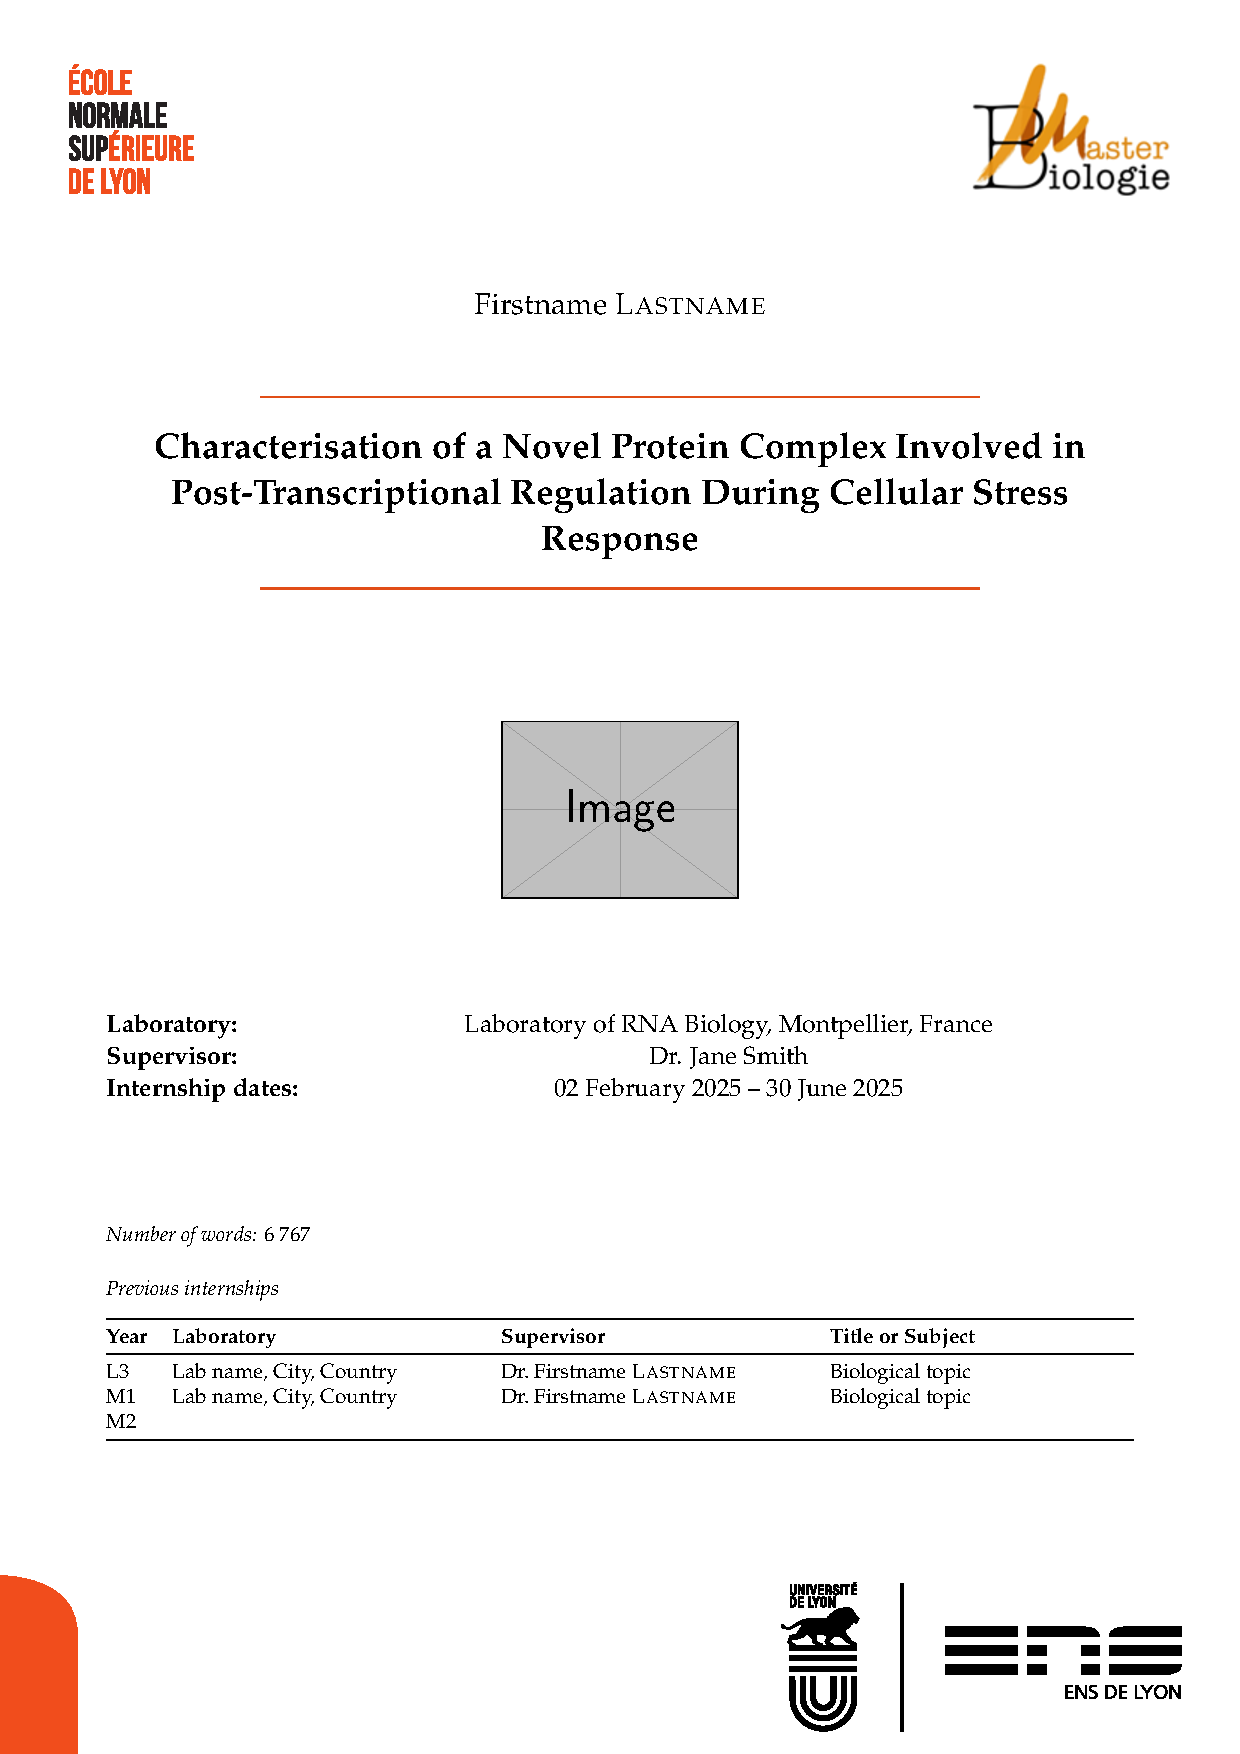
\includegraphics[page=1, width=0.72\linewidth]{enslyonstage-exemple.pdf}}\\[6pt]
  {\footnotesize\itshape Page de garde générée par \texttt{enslyonstage-exemple.tex} —
  thème \texttt{orange} (défaut).}
\end{center}

\newpage

% ═══════════════════════════════════════════════════════════════════════════
\section{Thèmes de couleur}
\label{sec:couleurs}
% ═══════════════════════════════════════════════════════════════════════════

\begin{demo}
\begin{lstlisting}[style=latexcode]
% Dans le préambule — choisir un thème :
\documentclass[orange]{enslyonstage}

% 22 thèmes disponibles :
% orange (défaut)  violet   blue
% red     green    teal     gray
% navy    azure    indigo   midnight
% slate   purple   pink     crimson
% wine    amber    gold     brown
% lime    forest   cyan
\end{lstlisting}
\tcblower
\footnotesize
\begin{tabular}{@{}lll@{}}
  \sw{E14D17}{orange}\,\textsuperscript{*} & \sw{652080}{violet}   & \sw{1A5C9E}{blue}    \\[3pt]
  \sw{A62020}{red}                          & \sw{1E6B3A}{green}    & \sw{0E6B6B}{teal}    \\[3pt]
  \sw{3A3A3A}{gray}                         & \sw{0D3B6E}{navy}     & \sw{1D4ED8}{azure}   \\[3pt]
  \sw{3730A3}{indigo}                       & \sw{1E2D5C}{midnight} & \sw{334155}{slate}   \\[3pt]
  \sw{5B21B6}{purple}                       & \sw{9D174D}{pink}     & \sw{881337}{crimson} \\[3pt]
  \sw{63152D}{wine}                         & \sw{92400E}{amber}    & \sw{7A5300}{gold}    \\[3pt]
  \sw{5C2D0E}{brown}                        & \sw{365314}{lime}     & \sw{14532D}{forest}  \\[3pt]
  \sw{0E6B8E}{cyan}                         &                       &                      \\
\end{tabular}\\[4pt]
{\itshape\footnotesize\textsuperscript{*}orange officiel ENS de Lyon — affecte titres, boîtes, citations et liens.}
\end{demo}


% ═══════════════════════════════════════════════════════════════════════════
\section{Structure du document}
% ═══════════════════════════════════════════════════════════════════════════

\subsection[\texttt{\textbackslash fairepagedegarde} et \texttt{\textbackslash faireabstract}]{\texttt{\textbackslash fairepagedegarde\{\}} et \texttt{\textbackslash faireabstract\{\}}}

\begin{demo}
\begin{lstlisting}[style=latexcode]
\begin{document}

% Génère la page de garde et
% bascule en mode deux colonnes
\fairepagedegarde

% Boîte abstract pleine largeur
% Doit suivre immédiatement
\faireabstract

% Table des matières (optionnel)
% \tableofcontents
\end{lstlisting}
\tcblower
\footnotesize
\begin{description}[noitemsep]
  \item[\texttt{\textbackslash fairepagedegarde}] Génère la page de garde officielle puis bascule automatiquement en mise en page \textbf{deux colonnes}.
  \item[\texttt{\textbackslash faireabstract}] Affiche l'abstract dans une boîte colorée \textbf{pleine largeur} en haut de la première page. Doit être appelé \textit{immédiatement} après.
  \item[\texttt{\textbackslash tableofcontents}] Optionnel. À retirer si le tuteur n'en demande pas.
\end{description}
\end{demo}

\newpage

% ═══════════════════════════════════════════════════════════════════════════
\section{Sections et titres}
% ═══════════════════════════════════════════════════════════════════════════

\subsection{\texttt{\textbackslash section\{\}}}

\begin{demo}
\begin{lstlisting}[style=latexcode]
\section{Introduction}
\label{sec:intro}
\end{lstlisting}
\tcblower
\simsection{Introduction}
\vspace{4pt}
{\footnotesize\itshape Fond coloré, centré, police sans-serif grasse. Le \texttt{\textbackslash label\{\}} permet les références croisées (\autoref{sec:refs}).}
\end{demo}

\subsection{\texttt{\textbackslash subsection\{\}}}

\begin{demo}
\begin{lstlisting}[style=latexcode]
\subsection{Contexte biologique}
\end{lstlisting}
\tcblower
\simsubsection[1.1]{Contexte biologique}
\vspace{4pt}
{\footnotesize\itshape Couleur principale, numérotation automatique.}
\end{demo}

\subsection{\texttt{\textbackslash subsubsection\{\}}}

\begin{demo}
\begin{lstlisting}[style=latexcode]
\subsubsection{Mécanismes moléculaires}
\end{lstlisting}
\tcblower
{\small\sffamily\bfseries 1.1.1\enspace Mécanismes moléculaires}
\vspace{4pt}
{\footnotesize\itshape À utiliser avec parcimonie dans un rapport de stage.}
\end{demo}

\subsection{\texttt{\textbackslash paragraph\{\}} — titres courants}

\begin{demo}
\begin{lstlisting}[style=latexcode]
\paragraph{Fly stocks and husbandry.}
Flies were maintained at
\qty{25}{\degreeCelsius} on standard
cornmeal–agar medium...

\paragraph{} % paragraphe sans titre
The \textit{Drosophila} wing imaginal
disc is a classical model...
\end{lstlisting}
\tcblower
\simparagraph{Fly stocks and husbandry.}
Flies were maintained at 25\,°C on standard cornmeal–agar medium\ldots\\[8pt]
\simparagraph{}
The \textit{Drosophila} wing imaginal disc is a classical model\ldots\\[6pt]
{\footnotesize\itshape \texttt{\textbackslash paragraph\{\}} est la commande standard pour les sous-parties de Matériels et Méthodes. 

Avec un argument vide, le titre est absent — utiliser pour faire un alinéa en début de section.}
\end{demo}

\newpage

\subsection{Sections non numérotées : \texttt{*}}

\begin{demo}
\begin{lstlisting}[style=latexcode]
\section*{Author Contributions}

\section*{Acknowledgements}
\end{lstlisting}
\tcblower
\simsectionstar{Author Contributions}
\vspace{2pt}
\simsectionstar{Acknowledgements}
\vspace{4pt}
{\footnotesize\itshape L'étoile \texttt{*} supprime la numérotation. À utiliser pour \textit{Author Contributions} et \textit{Acknowledgements}.}
\end{demo}

% ═══════════════════════════════════════════════════════════════════════════
\section{Listes — \texttt{itemize}, \texttt{enumerate}, \texttt{description}}
% ═══════════════════════════════════════════════════════════════════════════

\subsection{\texttt{itemize} — liste à puces}

\begin{demo}
\begin{lstlisting}[style=latexcode]
\begin{itemize}
  \item Imagerie confocale
  \item Séquençage ARN (RNA-seq)
  \item Relevés de biodiversité
\end{itemize}
\end{lstlisting}
\tcblower
\begin{itemize}[noitemsep, topsep=2pt]
  \item Imagerie confocale
  \item Séquençage ARN (RNA-seq)
  \item Relevés de biodiversité
\end{itemize}
\end{demo}

\subsection{\texttt{enumerate} — liste numérotée}

\begin{demo}
\begin{lstlisting}[style=latexcode]
\begin{enumerate}
  \item Extraire l'ARN total
  \item Synthétiser l'ADNc (RT)
  \item Amplifier par qPCR
  \item Normaliser sur gène de ménage
\end{enumerate}
\end{lstlisting}
\tcblower
\begin{enumerate}[noitemsep, topsep=2pt]
  \item Extraire l'ARN total
  \item Synthétiser l'ADNc (RT)
  \item Amplifier par qPCR
  \item Normaliser sur gène de ménage
\end{enumerate}
\end{demo}

\newpage

\subsection{\texttt{description} — termes définis}

\begin{demo}
\begin{lstlisting}[style=latexcode]
\begin{description}
  \item[Morphogène] Molécule de
    signalisation dont le gradient
    de concentration spécifie le
    destin cellulaire.
  \item[Imaginal disc] Épithélium
    larvaire de \textit{Drosophila}
    qui donne un organe adulte.
  \item[qPCR] PCR quantitative en
    temps réel ; mesure l'expression
    d'un gène cible.
\end{description}
\end{lstlisting}
\tcblower
\begin{description}[noitemsep, topsep=2pt, leftmargin=1.5em]
  \item[\textbf{Morphogène}] Molécule de signalisation dont le gradient de concentration spécifie le destin cellulaire.
  \item[\textbf{Imaginal disc}] Épithélium larvaire de \textit{Drosophila} qui donne un organe adulte.
  \item[\textbf{qPCR}] PCR quantitative en temps réel ; mesure l'expression d'un gène cible.
\end{description}
\end{demo}

\begin{astuce}
  Le package \texttt{enumitem} (déjà chargé par la classe) permet de personnaliser l'espacement :
  \texttt{[noitemsep]} supprime l'espace inter-items, \texttt{[topsep=2pt]} réduit l'espace au-dessus de la liste.
  Utile pour les légendes de figures ou les paragraphes Matériels et Méthodes.
\end{astuce}

% ═══════════════════════════════════════════════════════════════════════════
\section{Insérer une figure — \texttt{\textbackslash insererfigure}}
% ═══════════════════════════════════════════════════════════════════════════

\begin{demo}
\begin{lstlisting}[style=latexcode]
% Syntaxe générale :
\insererfigure[options]{fichier}
  {légende}{label}
\end{lstlisting}
\tcblower
\footnotesize
\begin{tabular}{@{}lp{4.8cm}@{}}
  \toprule
  \textbf{Argument} & \textbf{Contenu} \\
  \midrule
  \texttt{[options]} & Optionnel — voir ci-dessous \\
  \texttt{\{fichier\}} & Chemin de l'image (\texttt{figures/fig1.pdf}) \\
  \texttt{\{légende\}} & Texte de la légende \\
  \texttt{\{label\}} & Identifiant pour \texttt{\textbackslash autoref} (\texttt{fig:fig1}) \\
  \bottomrule
\end{tabular}
\end{demo}

\textbf{Options disponibles :}

\begin{center}
\footnotesize
\begin{tabular}{lp{7.5cm}l}
  \toprule
  \textbf{Option} & \textbf{Effet} & \textbf{Défaut} \\
  \midrule
  \textit{(aucune)} & Double colonne, placement \texttt{[!htb]} (à l'endroit dans le code) & \texttt{h=0.33\textbackslash textheight} \\
  \texttt{col}      & Colonne simple, \texttt{width=\textbackslash linewidth} & — \\
  \texttt{p}        & Page dédiée \texttt{[p]}, figure seule & — \\
  \texttt{b}        & Placement en bas de page (double colonne)  & — \\
  \texttt{h=<dim>}  & Hauteur personnalisée & \texttt{0.33\textbackslash textheight} \\
  \texttt{w=<dim>}  & Largeur personnalisée (remplace \texttt{h=}) & — \\
  \bottomrule
\end{tabular}
\end{center}

\begin{astuce}
  Préférez les images \textbf{vectorielles} au format \textbf{PDF} — elles
  restent parfaitement nettes à toute résolution et produisent un PDF final
  plus léger qu'un PNG/TIFF haute résolution. Pour vos graphiques
  (R, Python/matplotlib, Prism, Illustrator), exportez directement en
  \texttt{.pdf}. Pour les images de microscopie ou Western blot (données
  matricielles), le format \texttt{.tif} est recommandé.
\end{astuce}

\subsection{Figure double colonne (défaut)}

\begin{demo}
\begin{lstlisting}[style=latexcode]
% Occupe les deux colonnes
\insererfigure%
  {figures/fig1.pdf}%
  {\textbf{Titre de la figure.}
   (\textbf{A})~Schéma du protocole.
   (\textbf{B})~Résultats. $n = 7$,
   $p < 0.05$, test de Mann-Whitney.}%
  {fig:fig1}
\end{lstlisting}
\tcblower
\simfigbox[figures/fig1.pdf]{Titre de la figure. (\textbf{A})~Schéma du protocole. (\textbf{B})~Résultats. $n = 7$, $p < 0.05$, test de Mann-Whitney.}
\end{demo}

\subsection{Figure colonne simple — \texttt{[col]}}

\begin{demo}
\begin{lstlisting}[style=latexcode]
\insererfigure[col]%
  {figures/fig2.pdf}%
  {\textbf{Western blot.}
   Résultat de co-immunoprécipitation.}%
  {fig:coip}
\end{lstlisting}
\tcblower
{\footnotesize\itshape La figure est contenue dans \textbf{une seule colonne}. Idéal pour les petites figures ou les images dans une section à forte densité de texte.}\\[8pt]
{\footnotesize\textbf{Largeur} = \texttt{\textbackslash linewidth} (largeur d'une colonne).}
\end{demo}

\subsection{Figure pleine page — \texttt{[p]}}

\begin{demo}
\begin{lstlisting}[style=latexcode]
\insererfigure[p, w=0.9\textwidth]%
  {figures/fig3.pdf}%
  {\textbf{Réseau d'interaction.}
   Nœuds colorés par catégorie
   fonctionnelle.}%
  {fig:network}
\end{lstlisting}
\tcblower
{\footnotesize\itshape Crée une \textbf{page dédiée} à la figure (\texttt{[p]}). Idéal pour les grandes figures complexes avec beaucoup de panneaux.}\\[8pt]
{\footnotesize Combiner avec \texttt{w=} pour contrôler la largeur :\\
\texttt{w=0.9\textbackslash textwidth} = 90\,\% de la largeur du texte.}
\end{demo}

\newpage

\subsection{Largeur et hauteur personnalisées}

\begin{demo}
\begin{lstlisting}[style=latexcode]
% Largeur précise
\insererfigure[w=0.7\textwidth]
  {fig.pdf}{Légende}{fig:a}

% Hauteur précise
\insererfigure[h=0.25\textheight]
  {fig.pdf}{Légende}{fig:b}

% Double colonne, bas de page
\insererfigure[b]{fig.pdf}{Légende}{fig:c}
\end{lstlisting}
\tcblower
\footnotesize
\begin{description}[noitemsep]
  \item[\texttt{w=0.7\textbackslash textwidth}] La figure fait 70\,\% de la largeur totale du texte.
  \item[\texttt{h=0.25\textbackslash textheight}] La figure fait 25\,\% de la hauteur de la page.
  \item[\texttt{b}] Double colonne placée en bas de page de préférence.
  \item[\texttt{w=} et \texttt{h=}] Si les deux sont précisés, \texttt{w=} a priorité.
\end{description}
\end{demo}

\begin{astuce}
  Ajouter \verb|\FloatBarrier| après chaque sous-section pour empêcher les figures de migrer dans la section suivante (voir \autoref{sec:misc}).
\end{astuce}

\subsection{Structure d'une bonne légende}

\begin{demo}
\begin{lstlisting}[style=latexcode]
\insererfigure{figures/fig1.pdf}%
{%
\textbf{Titre en une phrase.}
(\textbf{A}) Description du panneau A.
(\textbf{B}) Description du panneau B.
$n = 7$ animaux par groupe.
Barres d'erreur = moyenne $\pm$ SEM.
*, $p < 0.05$ ; **, $p < 0.01$,
test de Mann-Whitney.%
}{fig:label}
\end{lstlisting}
\tcblower
\footnotesize\textbf{Éléments obligatoires :}
\begin{itemize}[noitemsep, topsep=2pt]
  \item Titre en \textbf{gras}, première phrase
  \item Description de chaque panneau (\textbf{A}), (\textbf{B})\ldots
  \item $n$ = nombre d'animaux/réplicats biologiques
  \item Test statistique et valeur de $p$ exacte
  \item Définition des barres d'erreur (SD, SEM\ldots)
  \item Définition des symboles (*, **)
\end{itemize}
\medskip
\itshape La légende doit être auto-suffisante.
\end{demo}

% ═══════════════════════════════════════════════════════════════════════════
\section{Figures supplémentaires — \texttt{\textbackslash inserersuppfig}}
% ═══════════════════════════════════════════════════════════════════════════

Les figures supplémentaires se placent \textbf{après} \verb|\biblio|, hors de la limite des 6~figures/tableaux ENS. Elles sont numérotées automatiquement S1, S2, \ldots\ (compteur indépendant) et s'étendent sur la pleine largeur du texte (\texttt{figure*}).

\medskip
\begin{astuce}
  Contactez \texttt{stages.biosciences@ens-lyon.fr} pour confirmer que votre tuteur ENS autorise les suppléments avant de les inclure.
\end{astuce}

\newpage

\subsection{Syntaxe de base}

\begin{demo}
\begin{lstlisting}[style=latexcode]
% Après \biblio — pleine largeur, numérotation S1, S2...
\inserersuppfig{figures/supp1.pdf}%
{%
  \textbf{Titre de la figure supplémentaire.}
  Description détaillée du panneau.
  $n = 5$ animaux. Barre d'échelle : \qty{10}{\micro\metre}.%
}{supp:fig1}
\end{lstlisting}
\tcblower
{\footnotesize\textbf{Arguments (dans l'ordre) :}
\begin{enumerate}[noitemsep, topsep=2pt]
  \item \texttt{[options]} — facultatif, options \verb|\includegraphics| (défaut : \texttt{width=\textbackslash textwidth})
  \item \texttt{\{fichier\}} — chemin de l'image
  \item \texttt{\{légende\}} — texte de légende (commence par titre en gras)
  \item \texttt{\{label\}} — étiquette pour \verb|\autoref{supp:fig1}|
\end{enumerate}
\medskip
Résultat : \textbf{Supplemental Figure~S1.}~Titre de la figure supplémentaire.\ldots}
\end{demo}

\subsection{Largeur personnalisée — argument optionnel}

\begin{demo}
\begin{lstlisting}[style=latexcode]
% Western blot : centré, largeur réduite à 60 %
\inserersuppfig[width=0.6\textwidth]{figures/supp_wb.pdf}%
{%
  \textbf{Western blot de contrôle.}
  Anti-PGK1 (contrôle de charge).
  Marqueurs de poids moléculaire (kDa) à gauche.%
}{supp:wb}
\end{lstlisting}
\tcblower
{\footnotesize\textbf{Tip :} passer \texttt{width=0.6\textbackslash textwidth} évite qu'un blot étroit ne paraisse flou une fois étiré à la pleine largeur.\medskip

Résultat : \textbf{Supplemental Figure~S2.}~Western blot de contrôle.\ldots}
\end{demo}

\subsection{Référence croisée}

\begin{demo}
\begin{lstlisting}[style=latexcode]
% Dans le corps du texte :
Voir \autoref{supp:fig1} pour les données de microscopie.
\end{lstlisting}
\tcblower
{\footnotesize Voir \textcolor{ENSorange}{\textbf{Supplemental Figure~S1}} pour les données de microscopie.\medskip

\textit{\texttt{\textbackslash autoref\{\}} reconnaît le compteur \texttt{suppfig} et formate automatiquement le renvoi.}}
\end{demo}

\newpage

% ═══════════════════════════════════════════════════════════════════════════
\section{Insérer un tableau}
% ═══════════════════════════════════════════════════════════════════════════

\subsection{Tableau double colonne — \texttt{table} / \texttt{table*}}

\begin{demo}
\begin{lstlisting}[style=latexcode]
% Caption AVANT le tabular (biologie)
% 'table'  = 1 colonne  |  'table*' = 2 colonnes
\begin{table}[!htb]
  \centering
  \caption{\textbf{Proteines identifiees.}
    $n = 3$ replicats. FC = fold-change.}
  \label{tab:partners}
  \small
  \begin{tabular}{llcc}
    \toprule
    \textbf{Proteine} & \textbf{Fonction}
      & \textbf{FC}  & \textbf{p} \\
    \midrule
    ProtA & ARN-binding & 4.2 & 0.001 \\
    ProtB & Stress gran. & 3.8 & 0.002 \\
    \bottomrule
  \end{tabular}
\end{table}
\end{lstlisting}
\tcblower
% \begin{table} est un flottant — non utilisable dans tcolorbox.
% On affiche directement le tabular avec une caption manuelle.
\begin{center}
\small \textbf{Table~1.} Proteines identifiees.
$n = 3$ replicats. FC = fold-change.\\[3pt]
\begin{tabular}{llcc}
  \toprule
  \textbf{Proteine} & \textbf{Fonction} & \textbf{FC} & \textbf{p} \\
  \midrule
  ProtA & ARN-binding & 4.2 & 0.001 \\
  ProtB & Stress gran. & 3.8 & 0.002 \\
  \bottomrule
\end{tabular}
\end{center}
\vspace{4pt}
\footnotesize\textbf{Règles clés :}
\begin{itemize}[noitemsep, topsep=2pt]
  \item \texttt{table*} = 2 colonnes, \texttt{table} = 1 colonne
  \item \texttt{\textbackslash caption} se place \textbf{au-dessus} du \texttt{tabular} (convention biologie)
  \item Toujours \texttt{booktabs} : \texttt{\textbackslash toprule \textbackslash midrule \textbackslash bottomrule}
  \item \texttt{\textbackslash small} ou \texttt{\textbackslash footnotesize} pour les tableaux denses
\end{itemize}
\smallskip
\textit{Tableaux et figures partagent le même quota : M1\,$\leqslant$\,6, M2\,$\leqslant$\,5.}
\end{demo}

% ═══════════════════════════════════════════════════════════════════════════
\section{Équations}
% ═══════════════════════════════════════════════════════════════════════════

\subsection{Équation numérotée — \texttt{equation}}

\begin{demo}
\begin{lstlisting}[style=latexcode]
Reaction velocity follows
Michaelis--Menten kinetics:
\begin{equation}
  v_i = \frac{v_\text{max}\,[S]}{K_m + [S]}
  \label{eq:mm}
\end{equation}

\noindent where $v_\text{max}$ is the
maximal velocity, $[S]$ the substrate
concentration and $K_m$ the Michaelis
constant.
\end{lstlisting}
\tcblower
Reaction velocity follows Michaelis--Menten kinetics:
\[
  v_i = \frac{v_{\text{max}}\,[S]}{K_m + [S]}
\]
\noindent where $v_{\text{max}}$ is the maximal velocity, $[S]$ the substrate concentration and $K_m$ the Michaelis constant.\\[6pt]
{\footnotesize\itshape \texttt{\textbackslash noindent} après l'équation empêche l'indentation du texte qui suit — indispensable quand on continue la phrase après une équation.}
\end{demo}

\subsection[Équation non numérotée]{Équation non numérotée — \texttt{equation*} ou \texttt{\textbackslash[\ldots\textbackslash]}}

\begin{demo}
\begin{lstlisting}[style=latexcode]
Henderson--Hasselbalch :
\begin{equation*}
  \text{pH} = \text{p}K_a
    + \log\frac{[\text{A}^-]}{[\text{HA}]}
\end{equation*}

% Forme courte équivalente :
\[ A = \varepsilon \cdot l \cdot c \]
\end{lstlisting}
\tcblower
Henderson--Hasselbalch :
\[
  \text{pH} = \text{p}K_a + \log\frac{[\text{A}^-]}{[\text{HA}]}
\]
\[ A = \varepsilon \cdot l \cdot c \]
{\footnotesize\itshape \texttt{equation*} et \texttt{\textbackslash[\,\textbackslash]} donnent le même résultat : une équation centrée sans numéro.}
\end{demo}

\subsection{Équations alignées — \texttt{align}}

\begin{demo}
\begin{lstlisting}[style=latexcode]
% Croissance logistique — membre gauche
% une seule fois, transformations du
% membre droit sur les lignes suivantes
\begin{align}
  \frac{dN}{dt}
    &= rN\!\left(1-\frac{N}{K}\right)
    \label{eq:logistic} \\
    &= rN - \frac{r}{K}\,N^2
    \label{eq:expanded}
\end{align}
\end{lstlisting}
\tcblower
\begin{align}
  \frac{dN}{dt}
    &= rN\!\left(1-\frac{N}{K}\right)
    \label{eq:logistic} \\
    &= rN - \frac{r}{K}\,N^2
    \label{eq:expanded}
\end{align}
{\footnotesize\itshape \texttt{align} aligne sur \texttt{\&}. Le membre gauche ($dN/dt$) n'apparaît qu'une fois : les lignes suivantes portent seulement \texttt{\&=} suivi de la forme développée. Chaque ligne peut avoir son propre \texttt{\textbackslash label\{\}}.\\[4pt]
Ici : modèle logistique ($N$ = effectif, $r$ = taux de croissance intrinsèque, $K$ = capacité biotique).}
\end{demo}

% ═══════════════════════════════════════════════════════════════════════════
\section{Bibliographie}
% ═══════════════════════════════════════════════════════════════════════════

\subsection{Déclarer la base de données — \texttt{\textbackslash addbibresource\{\}}}

\begin{demo}
\begin{lstlisting}[style=latexcode]
% Dans le préambule :
\addbibresource{references.bib}
\end{lstlisting}
\tcblower
{\footnotesize Le fichier \texttt{references.bib} contient vos références au format BibTeX/BibLaTeX. Sur Overleaf, \texttt{biber} est utilisé automatiquement.}\\[6pt]
{\footnotesize\textbf{Compilation locale :}\\
\texttt{pdflatex enslyonstage-gabarit} \textrightarrow{} \texttt{biber enslyonstage-gabarit} \textrightarrow{} \texttt{pdflatex enslyonstage-gabarit}}\\[6pt]
{\footnotesize\textit{Limite ENS : $\leqslant$ 35 références.}}
\end{demo}

\subsection{\texttt{\textbackslash cite\{\}} — citation simple}

\begin{demo}
\begin{lstlisting}[style=latexcode]
Comme démontré\cite{Vincent2020},
la protéine X s'assemble.

% Plusieurs références à la fois :
Résultats similaires\cite{Journo2021,Trizac2019,Vincent2020}.
% → compressé automatiquement en [1-3]
\end{lstlisting}
\tcblower
Comme démontré\simcite{1}, la protéine X s'assemble.\\[6pt]
Résultats similaires\simcite{1--3}.\\[8pt]
{\footnotesize\itshape Les citations apparaissent en exposant coloré. Les plages contigues sont compressées automatiquement : \texttt{\textbackslash cite\{A,B,C\}} donne \simcite{1--3} si les trois références sont numérotées consécutivement.}
\end{demo}

\subsection[\texttt{\textbackslash citeauthor} et \texttt{\textbackslash citeyear}]{\texttt{\textbackslash citeauthor\{\}} et \texttt{\textbackslash citeyear\{\}}}

\begin{demo}
\begin{lstlisting}[style=latexcode]
% Auteur visible dans la phrase :
Following \citeauthor{Vincent2020}%
\cite{Vincent2020}, we computed...

% Dans un tableau (source) :
\citeauthor{Vincent2020},
\citeyear{Vincent2020}
\end{lstlisting}
\tcblower
Following Nguyen et al.\simcite{1}, we computed\ldots\\[8pt]
Nguyen et al., 2020\\[8pt]
{\footnotesize\itshape Utile quand le nom de l'auteur fait partie de la phrase, ou dans les colonnes ``Source'' d'un tableau de souches/matériels.}
\end{demo}

\subsection{\texttt{\textbackslash biblio} — imprimer la bibliographie}

\begin{demo}
\begin{lstlisting}[style=latexcode]
% En fin de document :
\biblio
\end{lstlisting}
\tcblower
% Rendu réel via biblatex — refsection isole ces 3 entrées du .bib
% heading=none évite le \section* qui hérite du titleformat orange du README
\begin{refsection}
\nocite{Vincent2020}
\nocite{Journo2021}
\nocite{Trizac2019}
\nocite{Escarguel2015}
\nocite{Goudemand2019}
{\small\sffamily\bfseries References}\par\nopagebreak\vspace{2pt}
{\renewcommand*{\bibfont}{\tiny}\printbibliography[heading=none]}
\end{refsection}
\smallskip
{\scriptsize\itshape \texttt{\textbackslash biblio} ajoute également
«\,References\,» dans la table des matières.
Police \texttt{\textbackslash small} en style PNAS sans DOI — conforme
à l'exigence ENS.}
\end{demo}

\newpage

% ═══════════════════════════════════════════════════════════════════════════
\section{Références croisées}
\label{sec:refs}
% ═══════════════════════════════════════════════════════════════════════════

\subsection[\texttt{\textbackslash autoref} — référence colorée]{\texttt{\textbackslash autoref\{\}} — référence unique colorée}

\begin{demo}
\begin{lstlisting}[style=latexcode]
% Figure :
Voir \autoref{fig:fig1} pour le résultat.

% Section :
Les méthodes sont en \autoref{sec:methods}.

% Équation :
Tel que défini en \autoref{eq:mm}...

% Tableau :
Les données sont en \autoref{tab:data}.
\end{lstlisting}
\tcblower
Voir \simlink{Fig.~1} pour le résultat.\\[4pt]
Les méthodes sont en \simlink{Section~2}.\\[4pt]
Tel que défini en \simlink{Eq.~1}\ldots\\[4pt]
Les données sont en \simlink{Table~1}.\\[8pt]
{\footnotesize\itshape \texttt{\textbackslash autoref} génère automatiquement le préfixe coloré (``Fig.'', ``Table'', ``Section'', ``Eq.'') et crée un \textbf{lien cliquable} dans le PDF — un clic emmène directement à l'élément référencé.}
\end{demo}

\subsection[\texttt{\textbackslash crefcolor} — multi-références]{\texttt{\textbackslash crefcolor\{\}} — multi-références colorées}

\begin{demo}
\begin{lstlisting}[style=latexcode]
% Plusieurs figures d'un coup :
Voir \crefcolor{fig:fig1,fig:fig2}
pour les résultats principaux.

% Figures et tableaux mélangés :
\crefcolor{fig:fig1,tab:data}

% IMPORTANT — ne pas ajouter :
% \usepackage{cleveref}
% (déjà chargé par enslyonstage.cls)
\end{lstlisting}
\tcblower
Voir \simlink{Figs.~1 and~2} pour les résultats principaux.\\[6pt]
\simlink{Fig.~1 and Table~1}\\[8pt]
{\footnotesize\itshape \texttt{\textbackslash crefcolor} utilise \texttt{cleveref} pour gérer le pluriel et la liste automatiquement. \textbf{Ne pas ajouter} \texttt{\textbackslash usepackage\{cleveref\}} dans votre préambule : il est déjà chargé par la classe.}
\end{demo}

\begin{astuce}
  Toujours poser un \verb|\label{}| immédiatement après \verb|\section{}|,
  en 4\textsuperscript{e} argument de \verb|\insererfigure|, et après
  \verb|\begin{equation}|. Le label n'apparaît pas dans le PDF.\\[6pt]
  \textbf{Convention de nommage — \texttt{type:surnom}} : avant le
  \texttt{:} on indique la \emph{nature} de l'élément, après le \texttt{:}
  un surnom court et descriptif :
  \begin{itemize}[noitemsep, topsep=3pt]
    \item \texttt{fig:western}, \texttt{fig:results} — figures
    \item \texttt{tab:strains}, \texttt{tab:stats} — tableaux
    \item \texttt{sec:methods}, \texttt{sec:intro} — sections
    \item \texttt{eq:mm}, \texttt{eq:logistic} — équations
    \item \texttt{supp:confocal} — figures supplémentaires
  \end{itemize}
  \textbf{À éviter :} \texttt{fig1:western} ou \texttt{figure1} — sans
  préfixe standard, \texttt{\textbackslash autoref} ne peut pas
  déterminer le bon type et affichera le mauvais préfixe.
\end{astuce}

% ═══════════════════════════════════════════════════════════════════════════
\section{Unités — \texttt{siunitx}}
% ═══════════════════════════════════════════════════════════════════════════

\subsection{\texttt{\textbackslash qty\{\}\{\}} — valeur et unité}

\begin{demo}
\begin{lstlisting}[style=latexcode]
Vitesse : \qty{30}{\centi\metre\per\second}
Température : \qty{37}{\degreeCelsius}
Centrifugation : \qty{1500}{\rpm}
Concentration : \qty{5}{\milli\Molar}
Longueur d'onde : \qty{280}{\nano\metre}
Plage : \qtyrange{50}{100}{\micro\litre}
\end{lstlisting}
\tcblower
Vitesse : \qty{30}{\centi\metre\per\second}\\
Température : \qty{37}{\degreeCelsius}\\
Centrifugation : \qty{1500}{\rpm}\\
Concentration : \qty{5}{\milli\Molar}\\
Longueur d'onde : \qty{280}{\nano\metre}\\
Plage : \qtyrange{50}{100}{\micro\litre}\\[6pt]
{\footnotesize\itshape \texttt{\textbackslash rpm} et \texttt{\textbackslash Molar} sont des unités personnalisées déclarées dans la classe. Le séparateur entre unités est le point médian ($\cdot$) — exigence ENS.}
\end{demo}

\subsection{\texttt{\textbackslash unit\{\}} — unité seule}

\begin{demo}
\begin{lstlisting}[style=latexcode]
Toutes les longueurs sont en
\unit{\micro\metre}.

Unité composée seule :
\unit{\micro\gram\per\milli\litre}
\end{lstlisting}
\tcblower
Toutes les longueurs sont en \unit{\micro\metre}.\\[6pt]
\unit{\micro\gram\per\milli\litre}\\[6pt]
{\footnotesize\itshape Utiliser \texttt{\textbackslash unit\{\}} quand l'unité apparaît seule dans une phrase, sans valeur numérique.}
\end{demo}

\subsection{\texttt{\textbackslash num\{\}} — notation scientifique et grands nombres}

\begin{demo}
\begin{lstlisting}[style=latexcode]
Avogadro : \num{6.022e23}
Constante : \num{1.38e-23}
Population : \num{150000}
Enrichissement : \num{3.2}-fold
\end{lstlisting}
\tcblower
Avogadro : \num{6.022e23}\\
Constante : \num{1.38e-23}\\
Population : \num{150000}\\
Enrichissement : \num{3.2}-fold\\[6pt]
{\footnotesize\itshape \texttt{\textbackslash num} formate les nombres : séparateur de milliers, notation scientifique, alignement décimal.}
\end{demo}

\newpage

\subsection{Raccourcis personnalisés}

\begin{demo}
\begin{lstlisting}[style=latexcode]
% Définis dans le préambule de enslyonstage-gabarit.tex :
\newcommand{\um}{\unit{\micro\metre}}
\newcommand{\uM}{\unit{\micro\Molar}}
\newcommand{\degC}{\unit{\degreeCelsius}}

% Utilisation dans le texte :
Diamètre cellulaire : 10\,\um
Inhibiteur : \qty{2}{\uM}
Incubation : 37\,\degC
\end{lstlisting}
\tcblower
Diamètre cellulaire : 10\,\unit{\micro\metre}\\
Inhibiteur : \qty{2}{\micro\Molar}\\
Incubation : \qty{37}{\degreeCelsius}\\[8pt]
{\footnotesize\itshape Ajouter ses propres raccourcis dans la section ``CUSTOM SHORTCUTS'' du préambule de \texttt{enslyonstage-gabarit.tex}.}
\end{demo}

% ═══════════════════════════════════════════════════════════════════════════
\section{Formules chimiques — \texttt{mhchem}}
% ═══════════════════════════════════════════════════════════════════════════

\begin{demo}
\begin{lstlisting}[style=latexcode]
Peroxyde : \ce{H2O2}
Réaction ATP : \ce{ATP -> ADP + Pi}
Redox : \ce{NAD+ + H+ + 2e- -> NADH}
Ion : \ce{Ca^2+}, \ce{Mg^2+}
Radioisotope : \ce{^{32}P}
Buffer : \qty{50}{\milli\Molar} \ce{NaH2PO4}
\end{lstlisting}
\tcblower
Peroxyde : \ce{H2O2}\\
Réaction ATP : \ce{ATP -> ADP + Pi}\\
Redox : \ce{NAD+ + H+ + 2e- -> NADH}\\
Ion : \ce{Ca^2+}, \ce{Mg^2+}\\
Radioisotope : \ce{^{32}P}\\
Buffer : \qty{50}{\milli\Molar} \ce{NaH2PO4}\\[6pt]
{\footnotesize\itshape \texttt{\textbackslash ce\{\}} gère automatiquement les exposants/indices, les flèches de réaction et les équilibres.}
\end{demo}

% ═══════════════════════════════════════════════════════════════════════════
\section{Typographie — règles de style ENS}
% ═══════════════════════════════════════════════════════════════════════════

\subsection{Chiffres et nombres}

\begin{demo}
\begin{lstlisting}[style=latexcode]
% 1-9 sans unité : en lettres
We used three biological replicates
and observed 12 animals.

% Toujours en chiffres avec unité :
3 µm, 5 mM, \qty{10}{\micro\metre}

% Espace insécable avant une unité :
10~µm   % ou \qty{10}{\um}
\end{lstlisting}
\tcblower
\footnotesize
\begin{description}
  \item[1–9 sans unité] En lettres : \textit{three replicates}
  \item[10 et + sans unité] En chiffres : \textit{12 animals}
  \item[Avec unité] Toujours en chiffres : \textit{3\,µm}, \textit{5\,mM}
  \item[Espace insécable] \texttt{\textasciitilde} entre chiffre et unité écrite à la main ; géré automatiquement par \texttt{\textbackslash qty\{\}\{\}}
\end{description}
\end{demo}

\subsection{Italiques biologiques}

\begin{demo}
\begin{lstlisting}[style=latexcode]
% Gènes (italique) :
\textit{brca1}, \textit{TP53}, \textit{cdc28}

% Protéines (romain) :
BRCA1, p53, Cdc28

% Espèces (italique + espace insécable) :
\textit{S.~cerevisiae}, \textit{E.~coli}

% Locutions latines (italique) :
\textit{in vivo}, \textit{in vitro}
\end{lstlisting}
\tcblower
\footnotesize
\begin{description}[noitemsep]
  \item[Gènes] Italiques : \textit{brca1}, \textit{TP53}
  \item[Protéines] Romains : BRCA1, p53
  \item[Espèces] Italiques + espace insécable : \textit{S.~cerevisiae}
  \item[Latin] Italiques : \textit{in vivo}, \textit{in vitro}
\end{description}
\medskip
\itshape La tilde \texttt{\textasciitilde} dans \textit{S.\textasciitilde{}cerevisiae} empêche une coupure de ligne entre l'abréviation et le nom.
\end{demo}

\subsection{Signes typographiques}

\begin{demo}
\begin{lstlisting}[style=latexcode]
% Multiplication (pas la lettre x) :
$5 \times 10^6$ cellules

% Plus ou moins :
$12.3 \pm 0.4$~kDa

% Tiret demi-cadratin (plages) :
10--20\,\unit{\micro\metre}

% Tiret cadratin (incise) :
The complex --- as shown --- assembles.

% Environ :
$\approx \qty{300}{\nano\metre}$
\end{lstlisting}
\tcblower
$5 \times 10^6$ cellules\\[8pt]
$12.3 \pm 0.4$\,kDa\\[8pt]
10–20\,µm\\[8pt]
The complex --- as shown --- assembles.\\[8pt]
$\approx$ 300\,nm\\[12pt]
{\footnotesize
\texttt{-\,-} = tiret demi-cadratin – (plages)\\
\texttt{-\,-\,-} = tiret cadratin — (incise)\\
\texttt{\$\textbackslash times\$} = signe × (jamais la lettre x)}
\end{demo}

\subsection{Coupures de mots — \texttt{\textbackslash hyphenation\{\}}}

\begin{demo}
\begin{lstlisting}[style=latexcode]
% Dans le préambule de enslyonstage-gabarit.tex,
% pour les mots mal coupés :
\hyphenation{hy-po-gra-vi-ty
             quad-ru-pe-dal
             neu-ro-sciences}
\end{lstlisting}
\tcblower
{\footnotesize\itshape La classe applique déjà des pénalités d'hénation strictes (\texttt{\textbackslash hyphenpenalty=9900}) et protège les opérateurs mathématiques.\\[6pt]
Pour les termes techniques de votre domaine qui se coupent encore mal en bord de colonne, les ajouter dans \texttt{\textbackslash hyphenation\{\}} dans le préambule de \texttt{enslyonstage-gabarit.tex} : les tirets indiquent les coupures autorisées.}
\end{demo}

% ═══════════════════════════════════════════════════════════════════════════
\section{Mise en page avancée}
\label{sec:misc}
% ═══════════════════════════════════════════════════════════════════════════

\subsection{\texttt{\textbackslash FloatBarrier} — bloquer les flottants}

\begin{demo}
\begin{lstlisting}[style=latexcode]
\subsection{Résultats : partie A}
% ... figures et texte ...
\FloatBarrier
% Les figures précédentes ne passent
% pas au-delà de cette ligne

\subsection{Résultats : partie B}
\end{lstlisting}
\tcblower
{\footnotesize\itshape \texttt{\textbackslash FloatBarrier} (package \texttt{placeins}, déjà chargé) empêche les figures et tableaux de ``migrer'' au-delà de cette position. \textbf{Indispensable} pour garder les figures dans leur sous-section.\\[6pt]
Bonne pratique : placer un \texttt{\textbackslash FloatBarrier} à la fin de chaque sous-section de Résultats.}
\end{demo}

\subsection{\texttt{\textbackslash balance} — équilibrer la dernière page}

\begin{demo}
\begin{lstlisting}[style=latexcode]
% Juste avant \biblio :
\balance
\biblio
\end{lstlisting}
\tcblower
{\footnotesize\itshape \texttt{\textbackslash balance} (package \texttt{balance}, déjà chargé) égalise les hauteurs des deux colonnes sur la dernière page pour un rendu propre.\\[6pt]
À placer \textbf{juste avant} \texttt{\textbackslash biblio}, jamais plus tôt (cela peut perturber la mise en page des pages précédentes).}
\end{demo}

\subsection{\texttt{\textbackslash lettrine} — lettre ornée d'ouverture}

\begin{demo}
\begin{lstlisting}[style=latexcode]
\lettrine[lines=3]{D}{rosophila}
melanogaster has been a model organism
for studying developmental questions,
thanks to facilitated genetic
manipulations.
\end{lstlisting}
\tcblower
\lettrine[lines=3]{D}{rosophila} melanogaster has been a model organism for studying developmental questions, thanks to facilitated genetic manipulations.\\[6pt]
{\footnotesize\itshape Crée une grande lettre initiale sur \texttt{lines=3} lignes. Le package \texttt{lettrine} est déjà chargé par la classe. Premier argument = lettre ornée ; deuxième = suite de la lettre (en minuscules).}
\end{demo}

\newpage

\subsection[\texttt{\textbackslash TODO} et \texttt{\textbackslash NOTE} — annotations]{\texttt{\textbackslash TODO} et \texttt{\textbackslash NOTE} — annotations}

\begin{demo}
\begin{lstlisting}[style=latexcode]
\TODO{Vérifier les statistiques ici}

\NOTE{Cette figure vient du co-auteur}
\end{lstlisting}
\tcblower
{\color{red}\bfseries [TODO: Vérifier les statistiques ici]}\\[6pt]
{\color{ENSaccent}\itshape [NOTE: Cette figure vient du co-auteur]}\\[8pt]
{\footnotesize\itshape Ces commandes laissent des marqueurs visibles dans le PDF pendant la rédaction.}\\[4pt]
\begin{attention}
  {\footnotesize Supprimer \textbf{tous} les \texttt{\textbackslash TODO} et \texttt{\textbackslash NOTE} avant la soumission finale.}
\end{attention}
\end{demo}

\subsection{En-têtes et pieds de page — personnalisation}

\begin{demo}
\begin{lstlisting}[style=latexcode]
% Dans le préambule (optionnel) :
\coinhautgauche{Mon texte gauche}
\coinhautdroit{Mon texte droit}
\coinbasgauche{Mon texte gauche pied}
\coinbascentre{\includegraphics[height=8mm]
  {logos/custom.pdf}}
\coinbasdroit{Mon texte droit pied}
\end{lstlisting}
\tcblower
\footnotesize\textbf{Disposition par défaut (sans personnalisation) :}
\begin{description}[noitemsep]
  \item[Haut gauche] Nom de la section courante
  \item[Haut droit] Titre du rapport
  \item[Bas gauche] Domaine en petites capitales
  \item[Bas centre] Logo ENS à 8\,mm
  \item[Bas droit] Page\,/\,total
\end{description}
\medskip
\itshape Dans la grande majorité des cas, les valeurs par défaut conviennent. Ne personnaliser que si nécessaire.
\end{demo}

\newpage

% ═══════════════════════════════════════════════════════════════════════════
\section{Comptage de mots}
% ═══════════════════════════════════════════════════════════════════════════

\begin{demo}
\begin{lstlisting}[style=latexcode]
% La classe gère automatiquement
% les exclusions via des directives %TC: :

%TC:macro \insererfigure [0,0,0,0]
% → légendes de figures exclues

%TC:macro \abstracts [0]
% → abstract exclu

%TC:envir table  [0,0]
%TC:envir table* [0,0]
% → corps des tableaux exclus

% Sur Overleaf :
%   Menu → Word Count

% En local :
%   texcount -sum -1 enslyonstage-gabarit.tex
\end{lstlisting}
\tcblower
\footnotesize\textbf{Limites ENS :}\\
M1 : $\leqslant$ 5\,000 mots ($\pm$\,10\,\%)\\
M2 : $\leqslant$ 4\,000 mots ($\pm$\,10\,\%)\\[8pt]
\textbf{Exclusions automatiques :}
\begin{itemize}[noitemsep, topsep=2pt]
  \item Légendes de figures (\texttt{\textbackslash insererfigure})
  \item Corps et légendes des tableaux
  \item Abstract (\texttt{\textbackslash abstracts})
  \item Références bibliographiques
\end{itemize}
\medskip
\itshape Les directives \texttt{\%TC:} dans \texttt{enslyonstage.cls} sont lues par le compteur Overleaf et par \texttt{texcount} — aucune configuration supplémentaire n'est nécessaire.
\end{demo}


% ═══════════════════════════════════════════════════════════════════════════
\section{Exporter sa bibliographie \textit{Zotero} vers \LaTeX{}}
\label{sec:zotero}
% ═══════════════════════════════════════════════════════════════════════════

Le plug-in \textbf{Better \BibTeX} pour \textit{Zotero} génère des clés de citation stables
(format \texttt{AuteurAAAA}) et exporte votre bibliothèque au format \texttt{.bib}
directement utilisable avec \texttt{biblatex}/\texttt{biber}.

\subsection{Installer Better \BibTeX}

\begin{enumerate}
  \item Télécharger le fichier \texttt{.xpi} depuis\\
    \url{https://retorque.re/zotero-better-bibtex/installation/index.html}\\
    (cliquer sur le lien GitHub, puis télécharger le \texttt{.xpi}).
    \begin{center}
      \includegraphics[width=0.86\linewidth]{bibtex_site.png}
    \end{center}
    \begin{center}
      \includegraphics[width=0.70\linewidth]{bibtex_github.png}
    \end{center}
  \item Dans \textit{Zotero} : \texttt{Outils > Extensions}, puis roue dentée
    \textrightarrow{} \og Installer un plug-in à partir d'un fichier \fg,
    sélectionner le \texttt{.xpi} et redémarrer \textit{Zotero}.
    \begin{center}
      \includegraphics[width=0.70\linewidth]{zotero_extension.png}
    \end{center}
\end{enumerate}

\subsection{Gérer les clés de citation}

Ajouter une colonne \og clé de citation \fg{} dans \textit{Zotero} pour visualiser
et corriger les clés directement dans la bibliothèque.

\begin{center}
  \includegraphics[width=0.70\linewidth]{bibtex_citationkey.png}
\end{center}

\begin{astuce}
  Les clés suivent la convention \texttt{AuteurAAAA} (\textit{e.g.}
  \texttt{Vincent2020}), identique à celle utilisée dans \texttt{references.bib}.
  En cas de doublon, \textit{Better \BibTeX} ajoute automatiquement un suffixe
  (\texttt{Vincent2020a}, \texttt{Vincent2020b}\ldots).
\end{astuce}

\newpage

\subsection{Exporter le fichier \texttt{.bib}}

\texttt{Fichier > Exporter la bibliothèque}, choisir le format
\textbf{Better \BibTeX} ou \textbf{Better Bib\LaTeX}, cocher
\og Garder à jour \fg{} pour une synchronisation automatique, puis enregistrer
le fichier \texttt{.bib} dans le dossier du projet \LaTeX{}.

Déclarer ensuite le fichier dans le préambule :

\begin{lstlisting}[style=latexcode]
\addbibresource{nomdufichier.bib}

\end{lstlisting}

% ═══════════════════════════════════════════════════════════════════════════
\section{Questions fréquentes}
% ═══════════════════════════════════════════════════════════════════════════

\begin{description}[style=nextline]

  \item[\textit{Ma figure migre dans la mauvaise section.}]
    Ajouter \verb|\FloatBarrier| après la dernière figure de la sous-section.

  \item[\textit{La bibliographie ne compile pas sur Overleaf.}]
    Vérifier dans les paramètres du projet Overleaf que le compilateur est
    \texttt{pdfLaTeX} et le correcteur bibliographique \texttt{biber}
    (\textit{Menu → Compiler → LaTeX engine}).

  \item[\textit{La bibliographie ne compile pas en local.}]
    Respecter la séquence : \texttt{pdflatex main} → \texttt{biber main}
    → \texttt{pdflatex main}. Sur Overleaf, cette séquence est
    gérée automatiquement.

  \item[\textit{Erreur ``Undefined control sequence: \textbackslash crefcolor''.}]
    Ne pas ajouter \verb|\usepackage{cleveref}| dans le préambule : il est
    déjà chargé par \texttt{enslyonstage.cls}. Supprimer la ligne si elle
    est présente.

  \item[\textit{Le compteur de mots Overleaf est trop élevé.}]
    Vérifier que les figures sont insérées avec \verb|\insererfigure| (et
    non avec un environnement \texttt{figure} manuel) : la directive
    \texttt{\%TC:} de la classe n'exclut que \verb|\insererfigure|.

  \item[\textit{Mon logo de labo ne s'affiche pas.}]
    Vérifier que le fichier est dans le dossier \texttt{logos/}, que le
    chemin dans \verb|\logoLabo| est exact, et que la ligne est bien
    décommentée dans le préambule.

  \item[\textit{Le titre génère une erreur avec un saut de ligne.}]
    Utiliser \verb|\texorpdfstring{\\}{ }| à l'endroit du saut de ligne
    (voir \autoref{sec:metadata}).

  \item[\textit{Je veux changer de couleur de thème.}]
    Modifier l'option de \verb|\documentclass[blue]{enslyonstage}|.
    Les 22 thèmes disponibles sont listés en \autoref{sec:couleurs}.

  \item[\textit{La table des matières coupe une entrée en deux lignes.}]
    Corrigé en v2 (directive \verb|\nobreak| dans la classe). Si le
    problème persiste, raccourcir le titre ou utiliser la syntaxe
    \verb|\section[Titre court]{Titre long}|.

  \item[\textit{Les colonnes de la dernière page sont déséquilibrées.}]
    S'assurer que \verb|\balance| est placé \textit{juste avant}
    \verb|\biblio|, pas plus tôt dans le document.

\end{description}

\end{document}
